\section{Pc}
\subsection{GUI}
\begin{figure}[H]
\centering
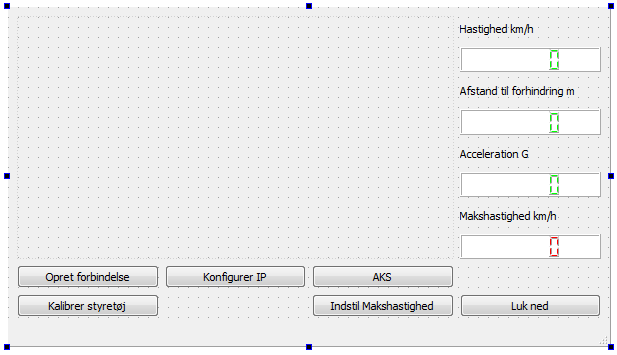
\includegraphics[width=\textwidth* 3/4,height=\textwidth* 9/20 ]{../fig/billeder/gui_design.png}
\caption{GUI i implementerings processen}
\label{fig:GUI_design}
\end{figure}
I denne sektion beskrives funktionerne i \texttt{MainWindow} i detaljer. Udviklingsmiljøet som hele GUI'en er skrevet i er Qt version 5.5 \cite{lib:qt}. En af fordelene ved QT er at man kan lave den grafiske del af GUI'en hurtigt og uden at skulle vide noget om hvordan koden bagved fungerer. Princippet er drag and drop og fungerer ved at man trækker de forskellige knapper og bokse ind i vinduet. Se figur \ref{fig:GUI_design}.
\subsubsection{MainWindow::MainWindow}
Qt opretter selv en klasse kaldet \texttt{MainWindow}. I main funktionen oprettes en instans af \texttt{MainWindow} som gør at hele programmet køres i MainWindow's constructor. Når programmet kører og der trykkes på en knap gives der et signal. Signalet forbindes til et slot i \texttt{constructoren} ved hjælp af funktionen \texttt{connect}. Hovedvinduets \texttt{signals and slots} forbindes i \texttt{constructoren}. I listing \ref{lst:constructor} ses fx. at når der klikkes på \texttt{OpretForbindelse} kaldes funktionen \texttt{Au2connect} som er funktionen der opretter forbindelsen til bilen. Det ses også at variablerne sættes til en default værdi samt der oprettes instanser af VLC-player når \texttt{constructoren} eksekveres. 
\begin{lstlisting}[caption={MainWindows constructor},label=lst:constructor, language=c++]
MainWindow::MainWindow(QWidget *parent)
    : QMainWindow(parent), ui(new Ui::MainWindow),media(0)
{
    isConnected=false;
    controllerConnected=false;
    ui->setupUi(this);
    this->setWindowTitle("Au2");

    instance = new VlcInstance(VlcCommon::args(), this);
    player = new VlcMediaPlayer(instance);
    player->setVideoWidget(ui->video);

    readDataFromFile();

    data[1] = 0;//hastighed
    data[2] = 0;//afstand
    data[3] = 0;//acceleration
    data[4] = 1;//AKS = on

    ui->AKS->setText("AKS-On");

    updateData();
    // Forbindelse af signals og slots 
    connect(ui->OpretForbindelse, SIGNAL(clicked()), this, SLOT(Au2connect()));
    connect(ui->KonfigurerIP, SIGNAL(clicked()), this, SLOT(konfigurerIP()));
    connect(ui->AKS, SIGNAL(clicked()), this, SLOT(AKSstatus()));
    connect(ui->IndstilMaksHastighed, SIGNAL(clicked()), this, SLOT(maksHastighed()));
    connect(ui->KalibrerStyretoj, SIGNAL(clicked()), this, SLOT(kalibrerStyretoj()));
    connect(ui->LukNed, SIGNAL(clicked()), this, SLOT(shutDown()));
    connect(this, SIGNAL(sig_getData()), this, SLOT(readSocket()));
}
\end{lstlisting}
\subsubsection{void MainWindow::Au2connect()}
Når \texttt{Au2connect} bliver kaldt testes der først om forbindelsen allerede er oprettet ved hjælp af variablen \texttt{isConnected}. Er forbindelsen allerede oprettet vil denne variabel være \textbf{true} og der gives besked til brugeren ved hjælp af en messageBox om at forbindelsen allerede er oprettet. Er forbindelsen ikke oprettet, oprettes \texttt{dataSocket} og \texttt{signals and slots} forbindes således signalet \texttt{connected} forbindes til funktionen \texttt{connected}, som sætter variablen \texttt{isConnected} til true samt skaber en messageBox hvor brugeren gives besked om at forbindelsen er oprettet. Derefter oprettes der forbindelse til bilen og der ventes indtil at forbindelsen er etableret, bliver forbindelsen ikke etableret oprettes en messageBox hvori bruger gives besked herom. Lykkedes det at oprette forbindelse kaldes funktionen \texttt{controller} som sørger for at forbinde controlleren med bilen. Når funktionen \texttt{controller} er returneret oprettes dataThread.
\begin{lstlisting}[caption={Au2Connect},label=lst:au2connect, language=c++]
void MainWindow::Au2connect()
{
    if(isConnected)
    {
        QMessageBox messageBox;
        messageBox.information(0,"Status","Forbindelsen er allerede oprettet!");
        messageBox.setFixedSize(500,200);
    }
    else
    {
        socket = new QTcpSocket(this);

        connect(socket,SIGNAL(connected()),this,SLOT(connected()),Qt::DirectConnection);
        connect(socket,SIGNAL(disconnected()),this,SLOT(connectionLost()),Qt::DirectConnection);

        socket->connectToHost(IP,1234);

        if(!socket->waitForConnected(1000))
        {
            QMessageBox messageBox;
            messageBox.critical(0,"Fejl","Forbindelsen blev ikke oprettet!");
            messageBox.setFixedSize(500,200);
        }
        else
        {
            controller();
            int error = pthread_create(&dataThread, NULL, this->getDataHelper ,this);
               if(error !=0)
              {
                qDebug()<<"Error on pthread_create"<<endl;
                return;
              }

            openPlayer();
         }
     }
}
\end{lstlisting}
\subsubsection{void MainWindow::controller()}
Funktionen \texttt{controller()} sørger for at forbinde controlleren med bilen. Der oprettes først en instance af \texttt{Xboxcontroller} hvorefter der testes om controlleren er forbundet. Er controlleren ikke forbundet oprettes der en messageBox hvori brugeren gives besked herom. Hvis controlleren er forbundet oprettes \texttt{controllerSocket} og dens \texttt{signals and slots} forbindes. Efterfølgende skabes der forbindelse og der testes om det lykkedes. Lykkedes det ikke gives bruger besked herom. Ellers oprettes \texttt{controllerThread} og funktionen returnerer. Se Listing \ref{lst:controller}.
\begin{lstlisting}[caption={controller},label=lst:controller, language=c++]
void MainWindow::controller()
{

    XboxController_ = new XboxController(1);

    if(!XboxController_->connect())
    {
        QMessageBox messageBox;
        messageBox.critical(0,"Fejl","Controlleren er ikke tilsluttet");
        messageBox.setFixedSize(500,200);
        delete XboxController_;
        return;
    }

    controllerSocket = new QTcpSocket;

    connect(controllerSocket,SIGNAL(connected()),this,SLOT(controllerIsConnected()),Qt::AutoConnection);
    connect(controllerSocket,SIGNAL(disconnected()),this,SLOT(controllerLostConnection()),Qt::AutoConnection);

    controllerSocket->connectToHost(IP,1235);

    if(!controllerSocket->waitForConnected(1000))
    {
        QMessageBox messageBox;
        messageBox.critical(0,"Fejl","Controlleren kunne ikke oprette forbindelse til bilen");
        messageBox.setFixedSize(500,200);
        delete controllerSocket;
        delete XboxController_;
    }
    else
    {
        int error = pthread_create(&controllerThread, NULL, this->controllerStreamHelper ,this);
           if(error !=0)
          {
            qDebug()<<"Error on pthread_create controller"<<endl;
            return;
          }

     }

}
\end{lstlisting}
\subsubsection{void* MainWindow::controllerStream()}
Funktionen \texttt{controllerStream()} streamer data fra controlleren til bilen således bilen kan reagere på input fra brugeren. Funktionen starter med at oprette et array hvori controller data gemmes. Data fra \texttt{XboxController} hentes og sendes til bilen ved hjælp af \texttt{controllerSocket} i en while-løkke, så længe \texttt{controllerConnected} er \textbf{true}.
\begin{lstlisting}[caption={controllerStream},label=lst:controller, language=c++]
void* MainWindow::controllerStream(void)
{
    char controllerData[4]={0};
    char turn;
    unsigned char forward;
    unsigned char back;
    bool brake;
    while (controllerConnected)
    {
        XboxController_->getCtrData(turn, forward, back, brake);
        controllerData[0]=forward;
        controllerData[1]=back;
        controllerData[2]=turn;
        controllerData[3]=(char)brake;
        controllerSocket->write(controllerData,4);
        controllerSocket->waitForBytesWritten();
        QThread::msleep(10);
    }

    return NULL;
}
\end{lstlisting}
\subsubsection{void* MainWindow::controllerStreamHelper()}
Funktionen \texttt{controllerStreamHelper} kaldes når \texttt{controllerThread} oprettes af \texttt{p\_thread\_create}. Da \texttt{p\_thread\_create} kun kan tilgå \texttt{static} funktioner gøres \texttt{controllerStreamHelper} \texttt{static} i \texttt{MainWindow.h}. Funktionen returnerer blot en pointer til \texttt{controllerStream}
\begin{lstlisting}[caption={controllerStream},label=lst:controller, language=c++]
void* MainWindow::controllerStreamHelper(void* context)
{
    return ((MainWindow *)context)->controllerStream();
}
\end{lstlisting}

\subsubsection{void* MainWindow::getData()}
Funktionen \texttt{getData} kører i en while-løkke så længe variablen \texttt{isConnected} er true. \texttt{isConnected} sættes til \textbf{true} når \texttt{dataSocket} har oprettet forbindelsen til bilen og false når \texttt{dataSocket} mister forbindelsen. I while-løkken gives signalet \texttt{sig\_getData} som gør at \texttt{MainWindow} eksekverer funktionen \texttt{readSocket} som sender og henter nyt data fra bilen. Efterfølgende eksekveres funktionen \texttt{updateData} som opdater variablerne i hovedvinduet.
\begin{lstlisting}[caption={getData},label=lst:getData, language=c++]
void* MainWindow::getData(void)
{
    while(isConnected)
    {
        sig_getData();
        updateData();
        QThread::msleep(100);
    }
    return NULL;
}
\end{lstlisting}
\subsubsection{void* MainWindow::getDataHelper()}
Funktionen \texttt{getDataHelper} kaldes når \texttt{dataThread} oprettes af \texttt{p\_thread\_create}. Da \texttt{p\_thread\_create} kun kan tilgå \texttt{static} funktioner gøres \texttt{getDataHelper} \texttt{static} i \texttt{MainWindow.h}. Funktionen retunerer blot en pointer til \texttt{getData}
\begin{lstlisting}[caption={getDataHelper},label=lst:getData, language=c++]
void* MainWindow::getDataHelper(void* context)
{
    return ((MainWindow *)context)->getData();
}
\end{lstlisting}

\subsubsection{void MainWindow::readSocket()}
Funktionen \texttt{readSocket} sender og læser data fra bilen. Når funktionen eksekveres låses \texttt{mutex} således andre funktioner ikke kan tilgå samme data.
\begin{lstlisting}[caption={readSocket},label=lst:readSocket, language=c++]
void MainWindow::readSocket()
{   
    mutex.lock();
    socket->write(data,6);
    socket->waitForBytesWritten();
    socket->waitForReadyRead();
    socket->read(data,6);
    mutex.unlock();
}
\end{lstlisting}

\subsubsection{void MainWindow::konfigurerIP()}
Funktionen \texttt{konfigurerIP} åbner for en inputdialog som giver brugeren mulighed for at indtaste en IP-adressen. IP-adressen gemmes i variablen \texttt{IP} og variablen \texttt{videoUrl} opdateres til stream-adressen fra bilen.
\begin{lstlisting}[caption={konfigurerIP},label=lst:konfigurerIP, language=c++]
void MainWindow::konfigurerIP()
{
    QString copy = IP;
    IP = QInputDialog::getText(this, tr("Konfigurer IP"), tr("Indtast IP adressen"), QLineEdit::Normal,IP);
    if (IP.isEmpty()){
    IP = copy;
    return;
    }
    videoUrl = "http://"+IP+":8081/stream.mjpeg";
}
\end{lstlisting}

\subsubsection{void MainWindow::AKSstatus()}
Funktionen \texttt{AKSstatus} ændre status på AKS på bilen. Når bruger trykker på knappen ''AKS-on'' ændres teksten til ''AKS-off'' og omvendt. Plads 4 i data arrayet opdateres til henholdsvis 1 eller 0. 
\begin{lstlisting}[caption={AKSstatus},label=lst:AKSstatus, language=c++]
void MainWindow::AKSstatus()
{
    data[4] =!data[4];
    if(data[4])
    ui->AKS->setText("AKS-On");
    else
    ui->AKS->setText("AKS-Off");
}
\end{lstlisting}

\subsubsection{void MainWindow::maksHastighed()}
Funktionen \texttt{maksHastighed} åbner en inputdialog hvor bruger gives mulighed for at indtaste en værdi mellem 0 og 10 i intervaller på 1. Alt uden for dette interval blokeres.  
\begin{lstlisting}[caption={maksHastighed},label=lst:maksHastighed, language=c++]
void MainWindow::maksHastighed()
{
    int copy = (int)data[0];
    bool ok;

    data[0] = (char)QInputDialog::getInt(this, tr("Makshastighed"),tr("Indtast makshastigheden"),
                                         (int)data[0], 0, 10, 1, &ok);
    if (!ok)
        data[0] = (char)copy;

    ui->lcdMakshastighed->display((int)data[0]);
}
\end{lstlisting}

\subsubsection{void MainWindow::writeDataToFile()}
Funktionen \texttt{writeDataToFile} åbner logfilen \texttt{Au2Data.txt} og skriver data arrayet til filen. Funktionen kaldes i \texttt{destructoren} således brugerinput gemmes når programmet lukkes. 
\begin{lstlisting}[caption={writeDataToFile},label=lst:writeDataToFile, language=c++]
void MainWindow::writeDataToFile()
{
    QFile file("Au2Data.txt");
        if(!file.open(QIODevice::WriteOnly))
            return;

    QTextStream out(&file);
    out << IP << "\r\n";
    out << videoUrl << "\r\n";
    out << (int)data[5] << "\r\n";
    out << (int)data[0] << "\r\n";
}
\end{lstlisting}

\subsubsection{void MainWindow::readDataFromFile()}
Funktionen \texttt{readDataFromFile} åbner logfilen \texttt{Au2Data.txt} og læser data arrayet fra filen. Funktionen kaldes i \texttt{constructoren} således brugerinput genindlæses ved opstart. 
\begin{lstlisting}[caption={readDataFromFile},label=lst:readDataFromFile, language=c++]
void MainWindow::readDataFromFile()
{
    QFile file("Au2Data.txt");
        if(!file.open(QIODevice::ReadOnly))
            return;

    QTextStream in(&file);
    IP = in.readLine();
    videoUrl = in.readLine();
    data[5] = (char)in.readLine().toInt();
    data[0] = (char)in.readLine().toInt();
}
\end{lstlisting}

\subsubsection{void MainWindow::kalibrerStyretoj()}
Funktionen \texttt{kalibrerStyretoj} åbner en inputdialog som giver brugeren mulighed for at indtaste en værdi mellem -50 og 50. Inputdialogen blokerer selv for værdier uden for dette interval.
\begin{lstlisting}[caption={kalibrerStyretoj},label=lst:kalibrerStyretoj, language=c++]
void MainWindow::kalibrerStyretoj()
{
    int copy = (int)data[5];
    bool ok;

    data[5] = (char)QInputDialog::getInt(this, tr("Styretoj"),tr("Indstil styretoj"),
                                         (int)data[5], -50, 50, 1, &ok);
    if (!ok)
        data[5] = (char)copy;
}
\end{lstlisting}

\subsubsection{void MainWindow::shutDown()}
Funktionen \texttt{shutDown} kaldes når GUI'en lukkes ned, enten i det røde kryds eller på knappen luk ned. Funktionen tester først om \texttt{dataSocket} er forbundet ved hjælp af variablen \texttt{isConnected}. Er der forbindelse låses \texttt{mutex} og der skrives \textbf{''dwnnow''} til bilen. Returneres dette igen fra bilen, har bilen accepteret at lukke ned. Hvis ikke dette modtages, åbnes en advarsel som giver bruger besked herom. Er forbindelsen ikke forbundet kaldes \texttt{MainWindows destructor} med funktionen \texttt{close}. 
\begin{lstlisting}[caption={shutDown},label=lst:shutDown, language=c++]
void MainWindow::shutDown()
{
    if(isConnected)
    {
        char sdata[6];
        mutex.lock();
        socket->write("dwnnow",6);
        socket->waitForBytesWritten();
        socket->waitForReadyRead();
        socket->read(sdata,6);
        if(sdata[0]=='d' && sdata[1]=='w' && sdata[2]=='n' && sdata[3]=='n' && sdata[4]=='o' && sdata[5]=='w')
        {
            socket->disconnect();
            mutex.unlock();
            close();
        }
        else
        {
            mutex.unlock();
            QMessageBox messageBox;
            messageBox.critical(0,"Fejl","Bilen kan ikke lukke ned!\n Prøv igen");
            messageBox.setFixedSize(500,200);
            return;
        }
    }
    close();
}
\end{lstlisting}

\subsubsection{void MainWindow::MainWindow()}
Dette er \texttt{MainWindows destructor} som først kalder \texttt{writeDataToFile} og derefter sletter oprettede instanser.
\begin{lstlisting}[caption={MainWindow},label=lst:MainWindow, language=c++]
MainWindow::~MainWindow()
{
    writeDataToFile();

    if(controllerSocket != NULL)
        delete controllerSocket;

    if(socket != NULL)
        delete socket;

    if(media != NULL)
        delete media;

    delete player;
    delete instance;
    delete ui;
}
\end{lstlisting}

\subsection{VLC}
Udviklingsmiljøet som hele GUI'en er skrevet i er Qt version 5.5. For at inkludere VLC, skal Qt være installeret \cite{lib:qt}. For at kunne modtage video stream i GUI'en skal vi bruge en forbygget version af VLC til windows32 indeholdende .dll filer osv, samt bilioteker til Qt. Dette gøres ved at udpakke Filen \textbf{vlc-2.0.7-win32.7z} som hentes fra en ftp server \cite{lib:vlc-ftp}. til destinationen \textbf{c:/Qt/}. Pakken indeholder rumtime-filerne som senere skal kopieres over i debugfolderen. Include filerne til Qt downloades \textbf{“Official VLC-Qt Windows SDK and Source Packages”} \cite{lib:vlc-qt} og udpakkes i \textbf{c:/Qt/}. I denne pakke ligger der et demoprojekt som der er hentet inspiration fra til projektet. Laves der et nyt projekt skal der inkluderes de rigtige filer til Qt. Dette gøres ved at åbne .pro filen i Qt og tilføje:

\begin{lstlisting}
# Edit below for custom library location
LIBS     += -LC:\Qt\libvlc-qt\lib -lvlc-qt -lvlc-qt-widgets
INCLUDEPATH += C:\Qt\libvlc-qt
\end{lstlisting}
Når projektet er bygget kopieres filerne \textbf{libvlc-qt-widgets.dll} og \textbf{libvlc-qt.dll} fra \textbf{C:/Qt/libvlc-qt/bin} til build folderen. Efterfølgende kopieres filerne \textbf{axvlc.dll, libvlc.dll, libvlccore.dll} og \textbf{npvlc.dll} fra \textbf{C:/Qt/vlc-2.0.7} samt folderen \textbf{plugins} også til buildfolderen. Programmet skulle nu genre kunne køre. Hvis ikke kan der findes mere hjælp her \cite{lib:vlc-using-qt}. Desværre er der nogle fejl i linket, som der gerne skulle være rettet i denne beskrivelse. 

\subsection{Test server}
Under udviklingsforløbet af GUI'en er der lavet en testserver som genererer tilfældigt data til GUI'en og udskriver på en terminal hvad der bliver modtaget fra GUI'en. Testserveren kan bruges til at teste alle funktioner i GUI'en. I listing \ref{lst:testserver,} ses \texttt{readReady} funktionen som reelt set står for funktionaliteten i serveren. Når der oprettes en testserver i main funktionen gives der i main en string med som parameter, som angiver om det er en data forbindelse eller controller forbindelse.
\begin{lstlisting}[caption={Læse og skrive funktionen i testserveren},label=lst:testserver, language=c++]
int Au2Thread::readyRead()
{
    COORD coord;
    HANDLE hConsole = GetStdHandle(STD_OUTPUT_HANDLE);

    if (type == "Data")
    {
    mutex->lock();
    char Data[6];

    /*
     data[0] = makshastighed
     data[1] = hastighed
     data[2] = afstand
     data[3] = acceleration
     data[4] = AKSstatus
     data[5] = styretoj
    */

    socket->read(Data,6);
    if(Data[0]=='d' && Data[1]=='w' && Data[2]=='n' && Data[3]=='n' && Data[4]=='o' && Data[5]=='w')
    {
        socket->write("dwnnow",6);
        coord.X = 0;
        coord.Y = 0;
        SetConsoleCursorPosition(hConsole, coord);
        QProcess::execute("CLS");
        std::cout << "System has been restarted"<<std::endl;
        std::cout << "Ready for new connection.."<< std::endl;
    }
    else
    {
        coord.X = 0;
        coord.Y = 5;
        SetConsoleCursorPosition(hConsole, coord);
        std::cout << "Recived data.. \r\n Makshastighed: "<< (int)Data[0]<<" Hastighed: "<< (int)Data[1]<<" Afstand: "
                     << (int)Data[2]<<" Acceleration: "<< (int)Data[3]<<" AKSstatus: "<< (int)Data[4]<<" Styretoj: "
                     << (int)Data[5]<<"    \r\n";
        char wData[6];
        wData[0]=Data[0];
        wData[1]=rand() % 100 + 1;
        wData[2]=rand() % 100 + 1;
        wData[3]=rand() % 100 + 1;
        wData[4]=Data[4];
        wData[5]=Data[5];
        std::cout << "Sending new data..    "<< "\r\n";
        socket->write(wData,6);
    }
    mutex->unlock();
    }
   else if (type == "Controller")
    {
        mutex->lock();
        char Data[4];
        socket->read(Data,4);
        /*
         data[0] = turn
         data[1] = speed
         data[2] = brake
        */
        coord.X = 0;
        coord.Y = 10;
        SetConsoleCursorPosition(hConsole, coord);
        std::cout << "Recived controller data.. \r\n Drej: "<< (int)Data[2]<<" Tilbage: "<< (int)(Data[1])<<" Frem: "<< (int)(Data[0])<<" Stop: "
                  << (int)Data[3]<<"            \r\n";
        mutex->unlock();
    }
    return 0;
}
\end{lstlisting} 
I figur \ref{fig:testserver} ses testserveren under test af GUI'en. 
\begin{figure}[H]
\centering
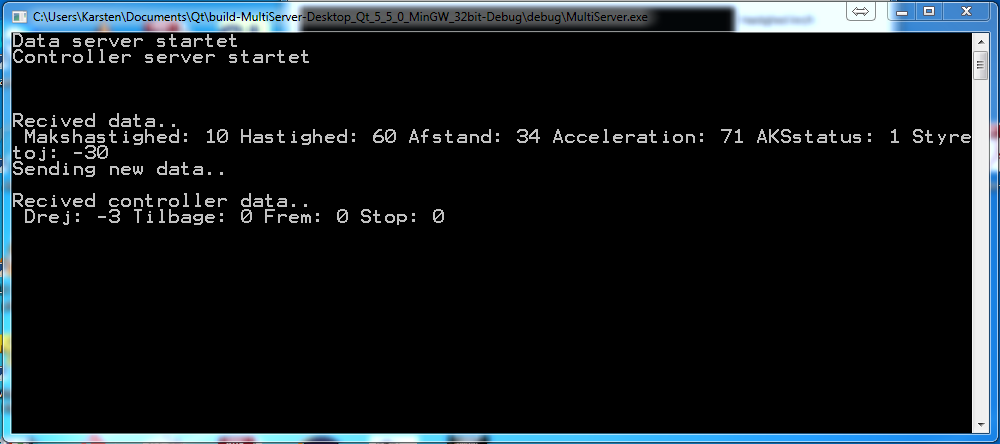
\includegraphics[width=\textwidth* 3/4,height=\textwidth* 8/20 ]{../fig/billeder/testserver.png}
\caption{Test server modtager data fra GUI}
\label{fig:testserver}
\end{figure}